%%%%%%%%%%%%%%%%%%%%%%%%%%%%%%%%%%%%%%%%%%%%%%%%%%%%%%%%%%%%%%%%%%%%%%%%%%%%%%%%%%%%%%
% Modelo de relatório de Disciplina de MLP a partir da
% classe latex iiufrgs disponivel em http://github.com/schnorr/iiufrgs
%%%%%%%%%%%%%%%%%%%%%%%%%%%%%%%%%%%%%%%%%%%%%%%%%%%%%%%%%%%%%%%%%%%%%%%%%%%%%%%%%%%%%%

%%%%%%%%%%%%%%%%%%%%%%%%%%%%%%%%%%%%%%%%%%%%%%%%%%%%%%%%%%%%%%%%%%%%%%%%%%%%%%%%%%%%%%
% Definição do tipo / classe de documento e estilo usado
%%%%%%%%%%%%%%%%%%%%%%%%%%%%%%%%%%%%%%%%%%%%%%%%%%%%%%%%%%%%%%%%%%%%%%%%%%%%%%%%%%%%%%
%
\documentclass[rel_mlp]{iiufrgs}

%%%%%%%%%%%%%%%%%%%%%%%%%%%%%%%%%%%%%%%%%%%%%%%%%%%%%%%%%%%%%%%%%%%%%%%%%%%%%%%%%%%%%%
% Importação de pacotes
%%%%%%%%%%%%%%%%%%%%%%%%%%%%%%%%%%%%%%%%%%%%%%%%%%%%%%%%%%%%%%%%%%%%%%%%%%%%%%%%%%%%%%
% (a A seguir podem ser importados os pacotes necessários para o documento, de acordo
% com a necessidade)
%
\usepackage[brazilian]{babel}	    % para texto escrito em pt-br
\usepackage[utf8]{inputenc}         % pacote para acentuação
\usepackage{graphicx}         	    % pacote para importar figuras
\usepackage[T1]{fontenc}            % pacote para conj. de caracteres correto
\usepackage{times}                  % pacote para usar fonte Adobe Times
\usepackage{enumerate}              % para lista de itens com letras
\usepackage{breakcites}
\usepackage{titlesec}
\usepackage{enumitem}
\usepackage{titletoc}
\usepackage{listings}			    % para listagens de código-fonte
\usepackage{mathptmx}               % p/ usar fonte Adobe Times nas formulas matematicas
\usepackage{url}                    % para formatar URLs
%\usepackage{color}				    % para imagens e outras coisas coloridas
%\usepackage{fixltx2e}              % para subscript
%\usepackage{amsmath}               % para \epsilon e matemática
%\usepackage{amsfonts}
%\usepackage{setspace}			    % para mudar espaçamento dos parágrafos
%\usepackage[table,xcdraw]{xcolor}  % para tabelas coloridas
%\usepackage{longtable}             % para tabelas compridas (mais de uma página)
%\usepackage{float}
%\usepackage{booktabs}
%\usepackage{tabularx}
%\usepackage[breaklinks]{hyperref}

\usepackage[alf,abnt-emphasize=bf]{abntex2cite}	% pacote para usar citações abnt

% isso meio que coloca helvetica no título dos capítulos, mas fica com muito espaçamento
%\titleformat{\chapter}
%  {\normalfont\fontsize{12}{0}\sffamily\bfseries}
%  {\thechapter}
%  {1em}
%  {}


% isso muda a fonte de tudo:
% \renewcommand\familydefault{\sfdefault}

%%%%%%%%%%%%%%%%%%%%%%%%%%%%%%%%%%%%%%%%%%%%%%%%%%%%%%%%%%%%%%%%%%%%%%%%%%%%%%%%%%%%%%
% Macros, ajustes e definições
%%%%%%%%%%%%%%%%%%%%%%%%%%%%%%%%%%%%%%%%%%%%%%%%%%%%%%%%%%%%%%%%%%%%%%%%%%%%%%%%%%%%%%
%

% define estilo de parágrafo para citação longa direta:
\newenvironment{citacao}{
    %\singlespacing
    %\footnotesize
    \small
    \begin{list}{}{
        \setlength{\leftmargin}{4.0cm}
        \setstretch{1}
        \setlength{\topsep}{1.2cm}
        \setlength{\listparindent}{\parindent}
    }
    \item[]}{\end{list}
}

% adiciona a fonte em figuras e tabelas
\newcommand{\fonte}[1]{\\Fonte: {#1}}

% Ative o seguinte caso alguma nota de rodapé fique muito longa e quebre entre múltiplas
% páginas
%\interfootnotelinepenalty=10000

%%%%%%%%%%%%%%%%%%%%%%%%%%%%%%%%%%%%%%%%%%%%%%%%%%%%%%%%%%%%%%%%%%%%%%%%%%%%%%%%%%%%%%
% Informações gerais
%%%%%%%%%%%%%%%%%%%%%%%%%%%%%%%%%%%%%%%%%%%%%%%%%%%%%%%%%%%%%%%%%%%%%%%%%%%%%%%%%%%%%%

% título
\title{Implementação de um Tower Defense com Swift}

% autor
%\author{Autor2}{Aluno} % {sobrenome}{nome} 1 para cada aluno
\author{Boranga}{Augusto} % {sobrenome}{nome}
\author{Franzoi Scroferneker}{Rodrigo} % {sobrenome}{nome}

% Professor orientador da disciplina
\advisor[Prof.~Dr.]{Mello Schnorr}{Lucas}

% Nome do(s) curso(s):
\course{Curso de Graduação em Ciência da Computa{\c{c}}{\~a}o e Engenharia de Computação}

% local da realização do trabalho
\location{Porto Alegre}{RS}

% data da entrega do trabalho (mês e ano)
\date{12}{2017}


% Palavras chave
\keyword{Palavra-chave1}
\keyword{Palavra-chave2}
\keyword{Palavra-chave3}


%%%%%%%%%%%%%%%%%%%%%%%%%%%%%%%%%%%%%%%%%%%%%%%%%%%%%%%%%%%%%%%%%%%%%%%%%%%%%%%%%%%%%%
% Início do documento e elementos pré-textuais
%%%%%%%%%%%%%%%%%%%%%%%%%%%%%%%%%%%%%%%%%%%%%%%%%%%%%%%%%%%%%%%%%%%%%%%%%%%%%%%%%%%%%%

% Declara início do documento
\begin{document}

% inclui folha de rosto
\maketitle

\selectlanguage{brazilian}

% Sumario
\tableofcontents



%%%%%%%%%%%%%%%%%%%%%%%%%%%%%%%%%%%%%%%%%%%%%%%%%%%%%%%%%%%%%%%%%%%%%%%%%%%%%%%%%%%%%
% Aqui comeca o texto propriamente dito
%%%%%%%%%%%%%%%%%%%%%%%%%%%%%%%%%%%%%%%%%%%%%%%%%%%%%%%%%%%%%%%%%%%%%%%%%%%%%%%%%%%%%

%espaçamento entre parágrafos
%\setlength{\parskip}{6 pt}

\selectlanguage{brazilian}



%%%%%%%%%%%%%%%%%%%%%%%%%%%%%%%%%%%%%%%%%%%%%%%%%%%%%%%%%%%%%%%%%%%%%%%%%%%%%%%%%%%%%
% Problema
%

\chapter{PROBLEMA} \label{intro}

Escolhemos para implementar o problema do jogo Tower Defense.

Tower Defense é um subgênero de jogos de estratégia, onde o jogador deve defender seu território (que varia de acordo com a temática do jogo) contra o ataque de inimigos, podendo utilizar um montante inicial para adquirir elementos do jogo que o ajudem na defesa.


%%%%%%%%%% Seção 1

\section{Dinâmica do jogo}

Basicamente, há dois elementos essenciais em um jogo do estilo Tower Defense:

\setlength{\itemindent}{1em}

    \item Territórios ou propriedades com certa quantidade de vida (o esgotamento desta implica em fim de jogo), que o jogador deve defender;

    \item Inimigos (com outra quantidade de vida) atacando os territórios do jogador;

\end{itemize}

A dinâmica do jogo com estes elementos é de que há "ondas" de ataques dos inimigos ao jogador. Isto é, o ataque ocorre em partes, com pequenas pausas entre eles.

O jogador pode então, entre ou durante as ondas de ataques (isto varia de jogo para jogo), utilizar-se de subterfúgios que atrapalhem a missão dos inimigos (como por exemplo, posicionar obstáculos ou outras estruturas que os ataquem). A aquisição destes equipamentos de defesa custa um certo valor que é decrementado do montante disponível para o jogador.

O objetivo do jogador é sobreviver ao final das N ondas de ataques inimigos.


\section{Historicamente}

Os primeiros jogos de Tower Defense datam da década de 1980, considerada a Era de Ouro dos video-games.

No jogo \textit{Space Invaders} - um clássico dos video-games lançado em 1978 -, o jogador deve defender seu território atirando em invasores alienígenas. É tido por uns como um precursor dos jogos de Tower Defense, mas isto é contestado por outros pelo fato de não possuir um elemento fundamental do gênero: a possibilidade de aquisição de elementos extras que auxiliem o jogador na defesa.

Já o jogo \textit{Rampart} - lançado em 1990 -, é amplamente considerado como o jogo que definiu o gênero, por possuir todos os elementos fundamentais deste. Em \textit{Rampart}, as fases de preparação (posicionamento dos itens de defesa), ação (momento em que a base é atacada e o jogador deve defendê-la) e reparação (consertar elementos danificados pelos ataques) são bem distintas.

\begin{figure}[htb]
    \centering
    \caption{Space Invaders, um dos pioneiros}
    \fbox{
        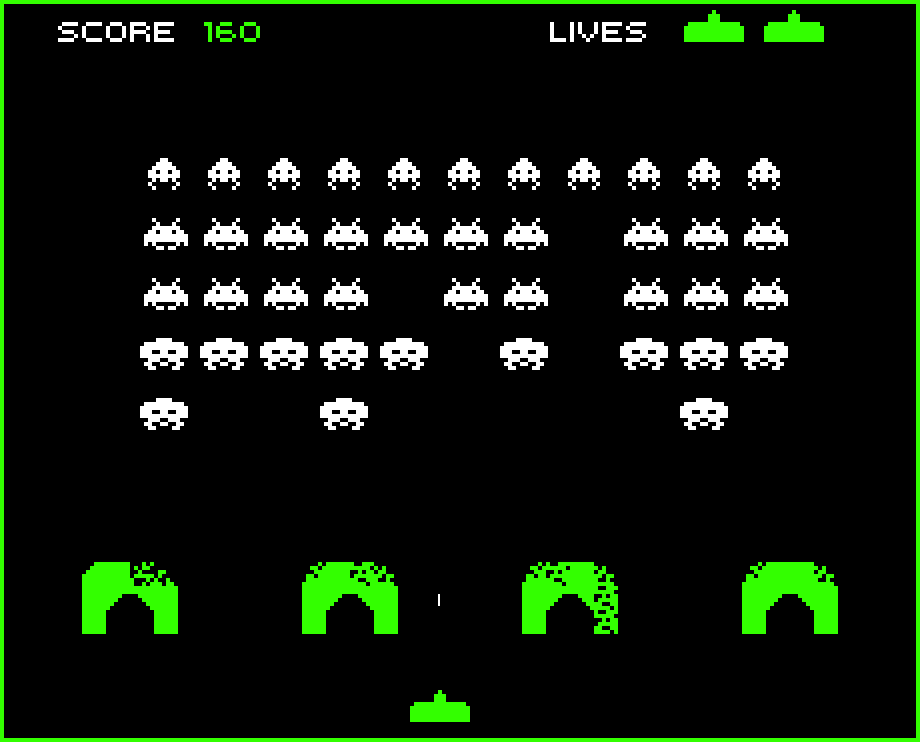
\includegraphics[width=12cm,height=8cm,keepaspectratio]{images/space-invaders.png}
    }
    \label{fig:figura1}
    \fonte{http://fantendo.wikia.com/wiki/File:Space-Invaders.png}
\end{figure}

\begin{figure}[htb]
    \centering
    \caption{Rampart, o Tower Defense clássico}
    \fbox{
        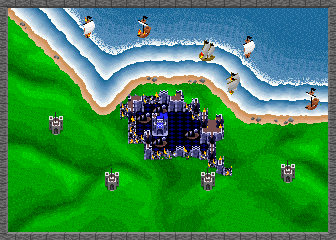
\includegraphics[width=12cm,height=8cm,keepaspectratio]{images/rampart.png}
    }
    \label{fig:figura1}
    \fonte{http://fantendo.wikia.com/wiki/File:Space-Invaders.png}
\end{figure}



%%%%%%%%%%%%%%%%%%%%%%%%%%%%%%%%%%%%%%%%%%%%%%%%%%%%%%%%%%%%%%%%%%%%%%%%%%%%%%%%%%%%%
% Linguagem
%

\chapter{LINGUAGEM} \label{intro}

Swift é uma linguagem de programação multiparadigma que se apresenta como uma linguagem moderna e focada em três aspectos: segurança, performance e suporte à aplicação de design patterns.

Mesmo sendo consideravelmente recente, Swift demonstra uma comunidade de bom tamanho, ficando em 11º nas linguagens mais populares e a 4ª mais amada no site stackoverflow em 2017.

Neste capítulo daremos um panorama a respeito da linguagem adotada, explanando acerca de suas origens e discutindo seus pontos positivos e negativos.


\section{História}

Swift é uma das linguagens de programação mais recentes desenvolvidas no mercado. Foi apresentada em 2014 na WWDC (Worldwide Developers Conference, evento organizado pela Apple para divulgação de novos produtos e features).

Baseada e influenciada por Objective-C, Ruby e Python, se mostrou uma linguagem poderosa e de fácil compreensão (devido principalmente, à sua sintaxe simples).

Inicialmente, Swift era de uso exclusivo por usuários de Mac OS, visto que este era o único sistema operacional habilitado a compilar a linguagem. Em dezembro de 2015, porém, um grande anúncio mudou o jogo: Swift viraria open source, abrindo um leque ainda maior de possibilidades de uso para a linguagem.


\section{Aspectos técnicos}

Swift é uma linguagem multiparadigma, suportando programação funcional e também oferecendo recursos de Orientação a Objetos, como classes e protocolos.

A linguagem possui tipagem estática, o que proporciona maior segurança (garantia dos tipos de dados esperados no código, evitando erros de tipos) e performance (não há gasto de máquina com checagem dos tipos) às aplicações que a utilizam.

Por ser construída pela Apple, possui alta integração com Obj-C, outra linguagem consagrada da Apple. Assim sendo, o programador que utiliza Swift tem à sua disposição uma série de bibliotecas em Obj-C, como por exemplo \textit{SpriteKit}, a biblioteca de construção de jogos que utilizaremos no desenvolvimento do trabalho.

Sua sintaxe foi pensada para ser o mais simples e expressiva possível, tornando o código mais fácil de ler e escrever.


\section{Utilização}

Mesmo sendo uma linguagem relativamente recente, Swift agradou a comunidade de desenvolvimento. Na pesquisa do site stackoverflow realizada em 2017, Swift ficou em 4º lugar nas linguagens preferidas pelos usuários.

Suas principais aplicações são:

\begin{itemize}[leftmargin=3em] % [label={--}]

\setlength{\itemindent}{1em}

    \item \textbf{Mobile}: Swift é a linguagem oficial para desenvolvimento de aplicativos para a plataforma iOS. Obj-C também é suportada em iOS, mas o programador mobile é encorajado pela própria Apple a utilizar Swift por esta ser uma linguagem mais recente e simples de usar;

    \item \textbf{Desktop}: Similar à plataforma mobile (citada acima), aplicações para o sistema operacional dos computadores da Apple (macOS, antigamente chamado OS X) também podem ser escritas em Swift;

    \item \textbf{Servidor}: Além disso, Swift também pode ser utilizado para o desenvolvimento de aplicações no lado do servidor. Existem alguns frameworks e toolkits (como o Perfect) que auxiliam o desenvolvedor nesta tarefa.

\end{itemize}

\section{Motivo da escolha}

Optamos por Swift por dois motivos:

\setlength{\itemindent}{1em}

    \item Ambos os integrantes do grupo tem familiaridade com a linguagem, devido a experiência prévia desenvolvendo aplicativos mobile.

    \item Swift é uma linguagem muito intuitiva e possui uma variedade de bibliotecas auxiliares disponíveis.

\end{itemize}

\section{Análise}

A análise crítica será feita ao término do trabalho.


%%%%%%%%%%%%%%%%%%%%%%%%%%%%%%%%%%%%%%%%%%%%%%%%%%%%%%%%%%%%%%%%%%%%%%%%%%%%%%%%%%%%%
% Capítulo 2
%
\chapter{IMPLEMENTAÇÃO}

Esta seção será construída no futuro.


%%%%%%%%%%%%%%%%%%%%%%%%%%%%%%%%%%%%%%%%%%%%%%%%%%%%%%%%%%%%%%%%%%%%%%%%%%%%%%%%%%%%%
% Conclusão
%
\chapter{CONCLUSÃO}

Esta seção será construída no futuro.


%%%%%%%%%%%%%%%%%%%%%%%%%%%%%%%%%%%%%%%%%%%%%%%%%%%%%%%%%%%%%%%%%%%%%%%%%%%%%%%%%%%%%
% Referências
%
\chapter{REFERÊNCIAS}

Esta seção será construída no futuro.

\end{document}
